
\chapter{Ukážky programov}
\label{kap:ukazky-programov}

V kapitole uvádzame niekoľko ukážok programov vytvorených v našej aplikácií. Tieto programy sú v nej k dispozícií pre začiatočníkov, ktorým môžu poskytnúť o niečo pohodlnejšiu štartovaciu pozíciu v procese zoznamovania sa s robotom a softvérom.

\section{Ultrazvukový senzor, čakanie}
Pre rýchle zoznámenie sa s možnosťami ultrazvukového senzora a významom súvisiaceho bloku pre \textit{čakanie} môže poslúžiť kód na obrázkoch \ref{obr:example-wave-on-proximity}, \ref{obr:example-wave-on-proximity-2}, \ref{obr:example-wave-on-proximity-3} a \ref{obr:example-wave-on-proximity-4}. Používateľ tak odhalí význam bloku \textit{čakania} a princíp nekonečného vyhodnocovania časti \textit{loop} riadiaceho programu. Program na obrázku \ref{obr:example-wave-on-proximity} predstavuje triviálnu implementáciu, robot máva rukou vždy, keď sa k nemu priblížime na menej ako pol metra. Ukážky \ref{obr:example-wave-on-proximity-2} a \ref{obr:example-wave-on-proximity-3} predstavujú zdanlivo identické programy, no aspekt \textit{čakania} z nich sémanticky robí celkom odlišné algoritmy. Ukážka na obrázku \ref{obr:example-wave-on-proximity-4} predstavuje alternatívny zápis programu v ukážke \ref{obr:example-wave-on-proximity-2}, používateľovi má priblížiť logický význam blokov pre \textit{čakanie}, \uv{čakanie je cyklické vykonávanie ničoho}.

\vspace{1cm}

\begin{figure}[h]
\centerline{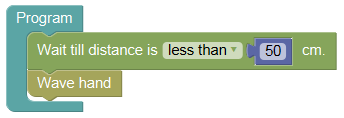
\includegraphics[width=0.6\textwidth]{images/example-wave-on-proximity}}
\caption[Ukážka programu --- zoznámenie s ultrazvukovým senzorom]{Ukážka programu --- zoznámenie s ultrazvukovým senzorom}
\label{obr:example-wave-on-proximity}
\end{figure}

\begin{figure}
\centerline{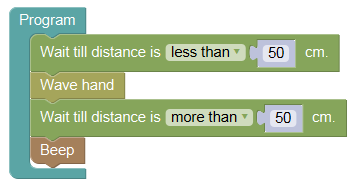
\includegraphics[width=0.6\textwidth]{images/example-wave-on-proximity-2}}
\caption[Ukážka programu --- zoznámenie s ultrazvukovým senzorom 2]{Ukážka programu --- zoznámenie s ultrazvukovým senzorom 2}
\label{obr:example-wave-on-proximity-2}
\end{figure}

\begin{figure}
\centerline{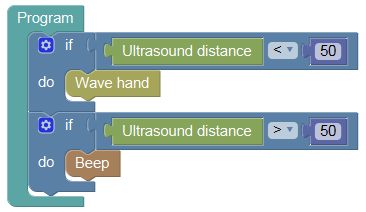
\includegraphics[width=0.6\textwidth]{images/example-wave-on-proximity-3}}
\caption[Ukážka programu --- zoznámenie s ultrazvukovým senzorom 3]{Ukážka programu --- zoznámenie s ultrazvukovým senzorom 3}
\label{obr:example-wave-on-proximity-3}
\end{figure}

\begin{figure}
\centerline{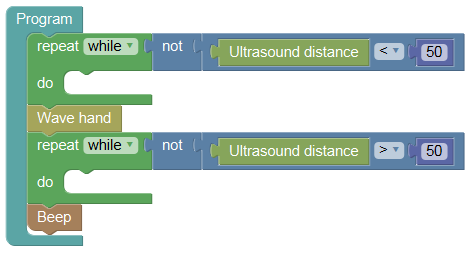
\includegraphics[width=0.8\textwidth]{images/example-wave-on-proximity-4}}
\caption[Ukážka programu --- zoznámenie s ultrazvukovým senzorom 4]{Ukážka programu --- zoznámenie s ultrazvukovým senzorom 4}
\label{obr:example-wave-on-proximity-4}
\end{figure}

\newpage

\section{Komplexný pohyb s detekciou prekážky}

Ukážka \ref{obr:avoid-collision} má za úlohu používateľovi v krátkosti ilustrovať využitie spojenia blokov pre pohyb, načítanie hodnoty zo senzora a cyklov. Praktický príklad ukazuje, ako sa možno na základe údajov o vzdialenosti vyhnúť blízkej prekážke.

\begin{figure}[h!]
\centerline{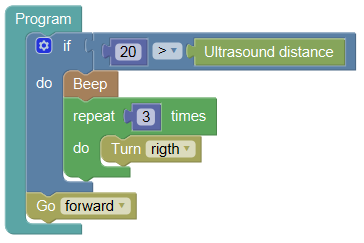
\includegraphics[width=0.58\textwidth]{images/avoid-collision}}
\caption[Ukážka programu \uv{vyhni sa prekážke}]{Ukážka programu \uv{vyhni sa prekážke}}
\label{obr:avoid-collision}
\end{figure}

\section{Výpis cez sériový port USB}

Ukážka \ref{obr:push-button} demonštruje, ako je možné jednoducho doplniť interakciu s robotom použitím sériovej komunikácie.

\begin{figure}[h!]
\centerline{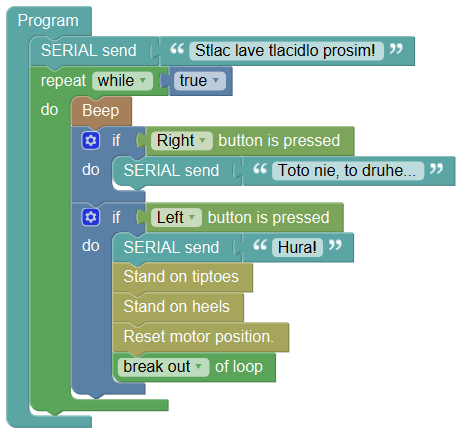
\includegraphics[width=0.58\textwidth]{images/push-button}}
\caption[Ukážka programu \uv{stlač ľavé tlačidlo}]{Ukážka programu \uv{stlač ľavé tlačidlo}}
\label{obr:push-button}
\end{figure}

\section{Funkcie a procedúry}
V nasledujúcej ukážke \ref{obr:guess-number} používateľa oboznamujeme s princípom procedúr a funkcií, ktoré môžu vo vhodnej forme uľahčiť čitateľnosť kódu. Program vždy vygeneruje náhodné číslo a nechá používateľa hádať. Ak uhádne, je vydaný \uv{oslavný} tón a vykonané jednoduché pohybové gesto. Ak je tip nesprávny, program reaguje odoslaním správy, či bol tip väčší alebo menší ako práve hádané číslo. V nenáročnom cvičení možno tento program prerobiť na tipovanie pomocou gesta rozpoznávaného senzorom alebo pridať implementáciu počítadla skóre.

\begin{figure}[h!]
\centerline{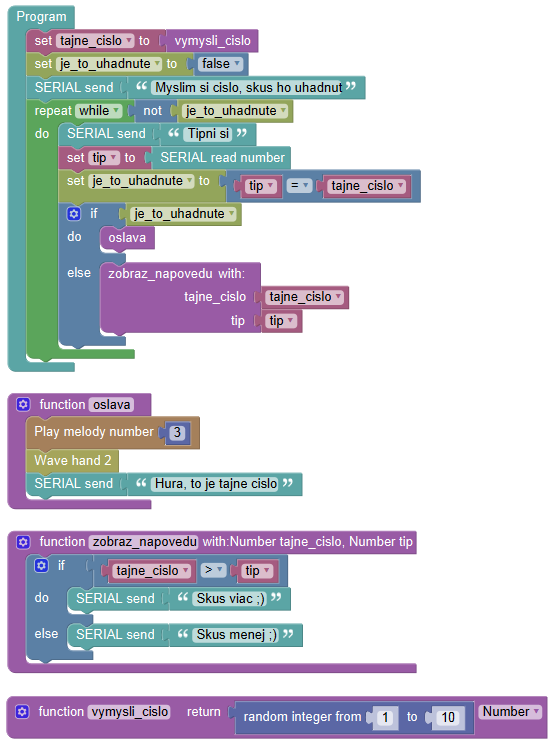
\includegraphics[width=0.8\textwidth]{images/guess-number}}
\caption[Ukážka programu \uv{hádaj číslo}]{Ukážka programu \uv{hádaj číslo}}
\label{obr:guess-number}
\end{figure}


















